%% Graph-based placement search over a heterogeneous accelerator cluster.
%%
%% TEMPORARY CLASS. `sigconf` with `nonacm` because no venue has been chosen
%% yet (P7.3 chooses it, and adjusting the template is a Claude Code task once
%% it has). `nonacm` suppresses the copyright block and the DOI/ISBN machinery
%% that an unsubmitted draft has no values for; removing it is the first edit
%% after a venue exists.
%%
%% BUILD: `make paper` from this directory. Do not run pdflatex by hand -- the
%% tables under tables/ are generated from experiments/results/*.md by
%% `make tables`, and a hand build silently compiles whatever was there last.
\documentclass[conference,10pt]{IEEEtran}
\usepackage{amsmath}
\usepackage{url}
\usepackage{adjustbox}
\usepackage{placeins}
%% IEEEtran asks for Times. Under pdfLaTeX that is its default; tectonic is
%% XeTeX, so the OpenType Times clone is named here, with its math and a
%% matching typewriter face. Named by file because tectonic resolves fonts
%% from its bundle, not from the system.
\usepackage{iftex}
\ifXeTeX
  \usepackage{fontspec}
  \setmainfont{texgyretermes}[Extension=.otf, UprightFont=*-regular,
    BoldFont=*-bold, ItalicFont=*-italic, BoldItalicFont=*-bolditalic]
  \setmonofont{texgyrecursor}[Extension=.otf, UprightFont=*-regular,
    BoldFont=*-bold, ItalicFont=*-italic, BoldItalicFont=*-bolditalic]
  \usepackage{unicode-math}
  \setmathfont{texgyretermes-math.otf}
\fi

\usepackage{booktabs}
\usepackage{tikz}
%% `positioning` is what makes `right=14mm of <node>` parse; without it
%% TikZ reads the phrase as arithmetic and fails on the word `of`.
\usetikzlibrary{positioning}
\usepackage{graphicx}

%% Generated tables are \input by name from sections/eval.tex. The search path
%% is set here so a section says \input{e_g1_toy_pilot} and not a relative path
%% that breaks when a section is moved.
\makeatletter
\providecommand\input@path{}
\g@addto@macro\input@path{{tables/}{figures/}}
\makeatother

%% `input@path` above is for `\input`; `\includegraphics` reads this one.
%% Without it a figure resolves only when the section happens to sit
%% beside it, which is not where sections live.
\graphicspath{{figures/}}

%% Every inline number in the body is a macro defined here, generated by
%% scripts/paper/numbers.py from experiments/results/*.md. `make check`
%% fails the build if a section contains a numeric literal instead.
%% GENERATED by scripts/paper/numbers.py. Do not edit.
%%
%% Every inline number in the paper is defined here, from a named cell
%% of a named results file. `make check` fails if a section contains a
%% numeric literal instead.

%% e_g5_real_hardware.md table 0 [all][agree]
\newcommand{\egfiveAgreeRows}{21}
%% e_g5_real_hardware.md table 0 [all][rows]
\newcommand{\egfiveAllRows}{27}
%% e_g5_real_hardware.md table 0 [condition-seeds whose answer changes][value]
\newcommand{\egfiveFloorChanged}{4}
%% e_g5_real_hardware.md table 0 [highest floor tried][value]
\newcommand{\egfiveFloorHigh}{1.6}
%% e_g5_real_hardware.md table 0 [lowest floor tried][value]
\newcommand{\egfiveFloorLow}{1.4}
%% e_g5_real_hardware.md table 0 [condition-seeds re-judged][value]
\newcommand{\egfiveFloorRows}{42}
%% e_g5_real_hardware.md table 0 [measured change][value]
\newcommand{\egfivePdEffect}{1.57}
%% e_g5_real_hardware.md table 0 [predicted change][value]
\newcommand{\egfivePdPredicted}{14.45}
%% e_g5_real_hardware.md table 0 [ratio][value]
\newcommand{\egfivePdRatio}{0.11}
%% e_g5_real_hardware.md table 0 [SD across pairs][value]
\newcommand{\egfivePdSd}{1.67}
%% e_g5_real_hardware.md table 0 [T1][original agrees]
\newcommand{\egfivePostToneOrigAgree}{8}
%% e_g5_real_hardware.md table 0 [T1][re-prediction agrees]
\newcommand{\egfivePostToneReAgree}{6}
%% e_g5_real_hardware.md table 0 [T1][rows]
\newcommand{\egfivePostToneRows}{10}
%% e_g5_real_hardware.md table 0 [T3][original agrees]
\newcommand{\egfivePostTthreeOrigAgree}{3}
%% e_g5_real_hardware.md table 0 [T3][original false positives]
\newcommand{\egfivePostTthreeOrigFp}{15}
%% e_g5_real_hardware.md table 0 [T3][re-prediction agrees]
\newcommand{\egfivePostTthreeReAgree}{17}
%% e_g5_real_hardware.md table 0 [T3][re-prediction false positives]
\newcommand{\egfivePostTthreeReFp}{0}
%% e_g5_real_hardware.md table 0 [T3][rows]
\newcommand{\egfivePostTthreeRows}{18}
%% e_g5_real_hardware.md table 0 [T1][reps]
\newcommand{\egfiveReps}{3}
%% e_g5_real_hardware.md table 0 [T1][goodput median]
\newcommand{\egfiveToneGoodput}{2.582}
%% e_g5_real_hardware.md table 0 [T1][p99 TTFT median]
\newcommand{\egfiveToneMedian}{404.5}
%% e_g5_real_hardware.md table 0 [T1][range]
\newcommand{\egfiveToneRangeHi}{421.3}
%% e_g5_real_hardware.md table 0 [T1][p99 TPOT median]
\newcommand{\egfiveToneTpot}{51.49}
%% e_g5_real_hardware.md table 0 [T3][disagree]
\newcommand{\egfiveTthreeDisagree}{6}
%% e_g5_real_hardware.md table 0 [T2][goodput median]
\newcommand{\egfiveTtwoGoodput}{2.445}
%% e_g5_real_hardware.md table 0 [T2][p99 TTFT median]
\newcommand{\egfiveTtwoMedian}{3341.1}
%% e_g5_real_hardware.md table 0 [T2][vs T1]
\newcommand{\egfiveTtwoOverTone}{8.3}
%% e_g5_real_hardware.md table 0 [T2][range]
\newcommand{\egfiveTtwoRangeLo}{3056.0}
%% e_g5_real_hardware.md table 0 [T2][p99 TPOT median]
\newcommand{\egfiveTtwoTpot}{56.20}
%% e_g5_real_hardware.md table 0 [normal][ratio to T1 at this level]
\newcommand{\egfiveWideHighRatio}{1.4}
%% e_g5_real_hardware.md table 0 [normal][ratio to T1 at this level]
\newcommand{\egfiveWideLowRatio}{1.1}
%% e_g5_real_hardware.md table 0 [normal][median p99 TTFT]
\newcommand{\egfiveWideTthreeLow}{394}
%% e_g4_microbench.md table 0 [all-reduce busbw, the TP=4 group][GB/s]
\newcommand{\egfourBusbwFour}{8.71}
%% e_g4_microbench.md table 0 [all-reduce busbw across the same bridge][GB/s]
\newcommand{\egfourBusbwTwo}{19.34}
%% e_g4_microbench.md table 0 [2][busbw plateau]
\newcommand{\egfourCollNicTwo}{5.07}
%% e_g4_microbench.md table 0 [2][busbw plateau]
\newcommand{\egfourCollNodeTwo}{19.34}
%% e_g4_microbench.md table 0 [as_measured][fluid]
\newcommand{\egfourFluidMeasuredBidi}{4.8}
%% e_g4_microbench.md table 0 [as_measured][fluid]
\newcommand{\egfourFluidMeasuredSame}{1.8}
%% e_g4_microbench.md table 0 [as_planned][fluid]
\newcommand{\egfourFluidPlannedSame}{93.1}
%% e_g4_microbench.md table 0 [single][median Gbit/s]
\newcommand{\egfourNicSingle}{88.61}
%% e_g4_microbench.md table 0 [two-same][median Gbit/s]
\newcommand{\egfourNicTwoSame}{44.36}
%% e_g4_microbench.md table 0 [as_measured][null]
\newcommand{\egfourNullMeasuredBidi}{48.3}
%% e_g4_microbench.md table 0 [as_planned][null]
\newcommand{\egfourNullPlannedSame}{7.5}
%% e_g4_microbench.md table 0 [peer copy across the PCIe bridge][GB/s]
\newcommand{\egfourPeerBridge}{25.12}
%% e_g4_microbench.md table 0 [peer copy over NVLink][GB/s]
\newcommand{\egfourPeerNvlink}{52.64}
%% e_g1_toy_pilot.md table 0 [graph-toy-asym][compression_ratio]
\newcommand{\egoneRatioAsym}{1.0}
%% e_g1b_topk.md table 0 [graph-toy-abcde][feasible_recall]
\newcommand{\egonebRecallGraphAbcde}{1.0}
%% e_g1b_topk.md table 0 [graph-toy-abcde][feasible_recall]
\newcommand{\egonebRecallSurrogateAbcde}{0.5}
%% e_g7_holdout.md table 0 [synth-holdout-1][embeddings]
\newcommand{\egsevenHoldoutEmbeddings}{36480}
%% e_g7_holdout.md table 0 [synth-holdout-1][compression_ratio]
\newcommand{\egsevenHoldoutRatio}{0.0164}
%% e_g7_holdout.md table 0 [synth-holdout-1][representatives]
\newcommand{\egsevenHoldoutReps}{600}
%% e_g6_scale.md table 0 [128][embeddings]
\newcommand{\egsixEmbeddingsLarge}{146688}
%% e_g6_scale.md table 0 [128][t_enumerate_s]
\newcommand{\egsixEnumerateLarge}{111}
%% e_g6_scale.md table 0 [128][compression_ratio]
\newcommand{\egsixRatioAsym}{0.067408}
%% e_g6_scale.md table 0 [128][compression_ratio]
\newcommand{\egsixRatioSym}{0.000286}
%% e_g6_real_sim.md table 0 [d32-s1.0][t_oracle_s]
\newcommand{\egsixRealOracleS}{38702}
%% e_g6_real_sim.md table 0 [d32-s1.0][oracle_simulations]
\newcommand{\egsixRealOracleSims}{9024}
%% e_g6_real_sim.md table 0 [d32-s1.0][t_proposed_s]
\newcommand{\egsixRealProposedS}{169}
%% e_g6_real_sim.md table 0 [d32-s1.0][proposed_simulations]
\newcommand{\egsixRealProposedSims}{42}
%% e_g6_scale.md table 0 [128][representatives]
\newcommand{\egsixRepsAsym}{9888}
%% e_g6_scale.md table 0 [128][representatives]
\newcommand{\egsixRepsSym}{42}
%% e_g3_real_sim_oracle.md table 0 [graph-toy-abcde][embeddings]
\newcommand{\egthreeEmbeddingsAbcde}{528}
%% e_g3_real_sim_oracle.md table 0 [heterogeneous-lab][embeddings]
\newcommand{\egthreeEmbeddingsLab}{114}
%% e_g3_real_sim_oracle.md table 0 [graph-toy-abcde][false_infeasible]
\newcommand{\egthreeFalseInfAbcde}{0}
%% e_g3_real_sim_oracle.md table 0 [graph-toy-abcde][compression_ratio]
\newcommand{\egthreeRatioAbcde}{0.1477}
%% e_g3_real_sim_oracle.md table 0 [heterogeneous-lab][compression_ratio]
\newcommand{\egthreeRatioLab}{0.6316}
%% e_g3_real_sim_oracle.md table 0 [graph-toy-abcde][representatives]
\newcommand{\egthreeRepsAbcde}{78}
%% e_g3_real_sim_oracle.md table 1 [graph-toy-abcde][saving_s]
\newcommand{\egthreeSavingAbcde}{2475}
%% e_g3_real_sim_oracle.md table 1 [heterogeneous-lab][saving_s]
\newcommand{\egthreeSavingLab}{269}
%% e_g3_real_sim_oracle.md table 1 [graph-toy-abcde][t_sim_oracle_s]
\newcommand{\egthreeSimOracleAbcde}{2790}
%% e_g3_real_sim_oracle.md table 1 [graph-toy-abcde][t_sim_proposed_s]
\newcommand{\egthreeSimProposedAbcde}{314}
%% e_g3_real_sim_oracle.md table 0 [graph-toy-abcde][unjudged]
\newcommand{\egthreeUnjudgedAbcde}{24}
%% e_g3_real_sim_oracle.md table 0 [heterogeneous-lab][unjudged]
\newcommand{\egthreeUnjudgedLab}{24}


%% A claim whose CLAIMS.md row is not `Established` is written in a form
%% that does not change when the result arrives, and marked with this.
%% The draft typesets a margin note; the final build redefines it to an
%% error, so a forgotten placeholder cannot be submitted.
%% The provenance tag that ends every table and figure caption. Rule 3:
%% MOCK, REAL SIM or REAL HARDWARE, so a figure read out of context
%% cannot be mistaken for a measurement it is not.
\newcommand{\sourcetag}[1]{\textsc{\footnotesize [#1]}}

\newcommand{\pending}[1]{\marginpar{\footnotesize PENDING: #1}}

\begin{document}

\title{Graph-Based Placement Search for Heterogeneous LLM Serving Clusters}

%% Placeholder. Replaced when the venue and the author list are settled (P7.3).
\author{\IEEEauthorblockN{Anonymous submission}}

\maketitle
%% ISPASS requires numbered pages; IEEEtran's conference mode omits them.
\thispagestyle{plain}
\pagestyle{plain}

\begin{abstract}
%% Every sentence here traces to a row of paper/CLAIMS.md. The hardware
%% sentence is deliberately the weakest one in the abstract, because the
%% strongest hardware result available is a failure.
Serving a large language model on a heterogeneous cluster means placing roles
on accelerators. Planners that enumerate configurations over interchangeable
devices conflate a configuration's placements, yet placement can decide whether
a latency target is met. We enumerate placements
and fold two only when graph isomorphism confirms that their candidate graphs,
which carry the shared communication boundary, agree. Elimination
relaxes the feasibility test, and a bounded budget reports what it never
evaluated. On hardware, one plan at two of its placements has a median $p99$
time to first token \egfiveTtwoOverTone{}x apart at the load knee. Against an
exhaustive simulated oracle on the largest toy fixture, \egthreeFalseInfAbcde{}
judged feasible placements were wrongly eliminated, and compression
saved \egthreeSavingAbcde{} of \egthreeSimOracleAbcde{} seconds. One result goes
against the model: across an inter-node NIC it predicted a
\egfivePdPredicted{}~ms slowdown of a disaggregated KV transfer; the hardware
showed \egfivePdEffect{}~ms, not distinguishable from zero.
\end{abstract}

%% Research design section 1 -- the judgement on the proposal, and what to claim as the paper's contribution.
%%
%% The three contributions, in the order the design fixes them:
%%   A  an equivalence relation over placements that carries the shared
%%      communication boundary, so two placements alike in every local
%%      attribute but differing in which contended uplink they cross are NOT
%%      folded together (evidence: E-G7's no_boundary arm);
%%   B  elimination that is a relaxation of the feasibility test, never a
%%      heuristic wearing the word "proved" (evidence: false_infeasible = 0
%%      across E-G1, E-G3, E-G5-boundary);
%%   C  an adaptive evaluation budget that reports what it never reached
%%      (evidence: E-G1b, E-G6, E-G7).
%%
%% Claims section 13 forbids and this section must not make: that this is the
%% first graph representation of a cluster (Helix), and that a Top-K procedure
%% guarantees a global optimum (heteropilot already has a Top-K).
\section{Introduction}
\label{sec:intro}

Serving a large language model on a heterogeneous cluster means choosing, for
one service specification, which accelerators run which role at which degree of
parallelism. The choice is a placement and not merely a configuration: two
groups of devices identical in model, memory and price can still differ in the
interconnect their tensor-parallel collective crosses, and that difference
reaches the served latency. Recent systems make that choice at cluster scale:
Helix~\cite{helix} places a model over heterogeneous GPUs and networks,
DistServe~\cite{distserve} and Splitwise~\cite{splitwise} split prefill and
decode across machines, and each group runs an engine such as
vLLM~\cite{vllm}.

% claim: C18
On the eight-GPU node used here, one plan---same engine, model, trace,
scheduler knobs and seed---deployed at two placements of itself has a median
$p99$ time to first token \egfiveTtwoOverTone{}x apart at the load knee, over
\egfiveReps{} repetitions per placement whose ranges do not overlap. Against a
latency target registered beforehand from the faster placement's own pilot, one
meets it and the other does not; Section~\ref{sec:eval} reports how the target
was chosen and how the ratio changes with load. A planner that enumerates
configurations rather than placements has no name for that choice. The planner
this work builds on is such a planner by construction: it maps a candidate to
an \emph{execution island} and hands the island's whole device list to the
runtime, so two placements of one candidate are, to it, one candidate.

% claim: C1
% claim: C3
Enumerating placements instead is expensive in evaluation, not enumeration:
each candidate's latency comes from a discrete-event simulation costing seconds
to minutes. The space is also redundant, because a cluster is built from
repeated parts, and the obvious response---hash a description of each
placement and evaluate one member per collision class---is where correctness
is lost silently. Two placements can agree in every local attribute and still
differ, because one crosses a link that something outside the deployment is
already using; a local signature merges them, and the evaluator's price for
the representative is attributed to both.

\paragraph{Contributions.}

% claim: C24
\textbf{A. An equivalence relation over placements that carries the shared
communication boundary.} Placements are folded only after a graph isomorphism
check confirms their candidate graphs agree, and those graphs carry the shared
resources their traffic crosses with the capacity each has left. Dropping the
boundary mis-merges the counterexample pair the relation exists for, which
the full relation does not.

% claim: C2
\textbf{B. Elimination that is a relaxation of the feasibility test.} A
candidate is removed only when arithmetic optimistic on every uncertain term
still misses a declared constraint, and each check publishes its relaxations;
anything else is reported as a heuristic, in a different state. In every
experiment that runs an exhaustive oracle the count of feasible placements
wrongly eliminated is zero among those the evaluator judged; on hardware the
bound is tested on one rejected candidate.

% claim: C11
% claim: C26
\textbf{C. An evaluation budget that reports what it did not reach.} The search
returns, with the recommendation, the representatives it never judged and the
placements they stand for. Under the real simulator the compression saved
\egthreeSavingAbcde~seconds against \egthreeSimOracleAbcde~seconds of oracle
simulation on the largest fixture, with its own hashing, isomorphism and bound
checks charged against it.

The work is built on an existing planner, and Table~\ref{tab:reuse} says which
parts are reused, which are modified through hooks, and which are new. It does
not claim to be the first graph representation of a serving cluster, nor that
a top-$K$ procedure yields a global optimum.

%% Research design sections 10 and 15 -- what already exists, and the reading
%% order of the code it exists in.
%%
%% Carries the reuse-vs-contribution boundary table that P6.2 makes mandatory:
%% heteropilot modules (planner.inventory, candidate_generator, predictor,
%% optimizer, deploy) / graphsearch modules (schema, paths, demand, embeddings,
%% equivalence, bounds, ranker, adaptive, adapter, restore, oracle, cost,
%% contention) / the hooks H1-H4. A reader must be able to tell, per claim,
%% which repository the code is in.
\section{Background}
\label{sec:background}

\input{reuse}

\paragraph{Execution islands.}
The planner this work extends describes a cluster as a set of \emph{execution
islands}: maximal groups of accelerators of one model, joined by one kind of
intra-island interconnect, that can host a single serving engine. A candidate
names an island and a parallelism degree; the deployer resolves the island to
its device list and lets the runtime take the devices it needs. That
abstraction is already an unstated compression: it collapses every placement
within an island into one candidate, which is sound exactly when the island's
devices are interchangeable. They are, in model and memory, by definition; they
are not necessarily interchangeable in what their traffic crosses. The
planner's own envelope cache, which shares a prediction between configurations
whose \emph{twin} keys agree, is a different and deliberately approximate
merge, and is not replaced here.

\paragraph{The simulator.}
Latency predictions come from LLMServingSim~\cite{llmservingsim,llmservingsim2},
a discrete-event simulator built on ASTRA-sim~\cite{astrasim,astrasim2} and
its Chakra traces~\cite{chakra}, here with an analytical network backend. It accepts a link bandwidth and a latency per collective and
has no representation of a link graph, so it cannot be told that two groups
share a wire (Section~\ref{sec:adapter}).

\paragraph{What is reused and what is new.}
The inventory, candidate generator, predictor interface, optimiser and
deployment backends are the existing planner's. Four hooks were added to it,
in its own repository and each a numbered deviation there; they touch some of
those modules, and with no hook in use the planner behaves as before; the graph
representation, equivalence, elimination, ranking, adaptive budget, simulator
adapter and restoration are new (Table~\ref{tab:reuse}). No behaviour of the
existing planner changes when the hooks are not used, which its own golden
tests check.

%% Research design section 2 -- the optimisation problem and what a candidate is.
%%
%% Two things this section has to establish before anything later can be said:
%% a candidate is a complete executable plan (placement + parallelism + roles +
%% knobs + routing), not a device subset; and the inputs are not exhausted by
%% the interconnect and the SLO -- the contract needs goodput and cost too,
%% which is what heteropilot's H1 hook added (slo.min_goodput_rps).
\section{Problem statement}
\label{sec:problem}

\paragraph{Inputs.}
A service specification fixes the model and dtype, the traffic (arrival rate,
burstiness, token distributions) and the service level objectives: a
percentile and a limit for time to first token and for time per output token,
and, when the operator states one, a minimum goodput. A cluster specification
fixes the nodes, their accelerators with model, memory and price, the links
with bandwidth, latency and direction, and the resources several links contend
for, each with a capacity and the share already reserved by traffic this
planner does not control.

\paragraph{Candidates and objective.}
A candidate is a complete plan: which devices run which role at which tensor-
and pipeline-parallel degree, with how many replicas, under which scheduler
knobs and routing policy. Two candidates that differ only in which devices
they occupy are two candidates. The objective is minimum cost per hour among
candidates that meet every declared constraint; a plan touching an unpriced
device is reported as uncomputed rather than scored on a partial sum.

% claim: C2
% claim: C3
\paragraph{Five states, which never merge.}
Every candidate ends in exactly one of five states:
\textbf{\texttt{impossible\_proven}} (optimistic arithmetic still misses a
declared constraint), \textbf{\texttt{excluded\_by\_scope}} (removed by a
budget or a stated scope cut), \textbf{\texttt{deferred\_heuristic}} (rejected
by a rule that cannot be shown to be a relaxation, and not called proved),
\textbf{\texttt{unknown\_measurement}} (the evaluator was asked and did not
answer), and \textbf{\texttt{evaluated}}. \emph{Unevaluated is not
infeasible}: a search that silently omits what it never reached has made a
claim about the whole space on evidence from part of it, so every result
reports how many representatives went unjudged and how many placements they
stand for.

\paragraph{Two correctness numbers.}
\texttt{false\_infeasible} counts candidates the search eliminated that an
exhaustive oracle finds feasible, and \texttt{mismerged\_pairs} counts pairs of
placements folded into one representative that the oracle prices differently.
Both must be zero. They are conditions, not scores: a non-zero value is a
broken invariant, and the registered response is to stop and report.

%% Research design section 3 -- the physical graph and the communication demand
%% expressed together.
%%
%% graphsearch/schema.py (normalisation: bytes/s throughout, directed edges,
%% shared resources as vertices), graphsearch/paths.py (allowed paths, cut
%% capacity, the boundary), graphsearch/demand.py (CommFlow).
%%
%% The unit trap of section 3 belongs here and is not a footnote: a link's
%% datasheet gbps, a collective's busbw and the simulator's link_bw answer
%% different questions, and heteropilot's A40 bridge measures 25.0 / 19.29 /
%% 8.8 GB/s for one wire depending on which is asked.
\section{Representing the cluster and its traffic}
\label{sec:graph}

\paragraph{One graph, normalised.}
The cluster becomes a directed graph whose vertices are accelerators, network
interfaces, CPU sockets and switches, and whose edges are links. Every capacity
is bytes per second, whatever unit the source file used; a schema that lets one
file mean gigabytes and another gigabits is a schema in which a factor of eight
survives review. Undirected links in the source become two directed edges, so a
path is a sequence of edges and not a sequence of ambiguous adjacencies.

\paragraph{Shared resources are vertices, not annotations.}
A resource that several links contend for---a host bridge, an uplink, a switch
port---enters the graph as its own vertex, with the links that cross it
incident on it. It carries a capacity and the share already reserved by traffic
outside this deployment. Making it a vertex rather than a label is what lets a
cut computation see it: the capacity between two device sets is then a maximum
flow in a graph where the contended element is a real node with a real
capacity, and a reservation is subtracted before any bound is computed rather
than after.

\paragraph{Demand.}
A candidate's traffic is a set of flows, each with its participants, its bytes
per event, its events per request, and whether a latency target charges for it.
The last field is load-bearing: ingress and egress cross an uplink and consume
its capacity, but no declared SLO charges for their time, so a model that
priced only what the SLO charges for would conclude that those flows are free
and that the uplink they saturate is idle.

\paragraph{A link does not have \emph{a} bandwidth.}
This is the trap the representation exists to avoid, and it is not a footnote.
One wire answers different questions with different numbers depending on what
crosses it. Measured on the eight-GPU node used in
Section~\ref{sec:eval}, one PCIe path between two accelerators sustains
\egfourPeerBridge~GB/s for a direct peer copy, \egfourBusbwTwo~GB/s of bus
bandwidth for a two-rank all-reduce, and \egfourBusbwFour~GB/s for the
four-rank all-reduce a tensor-parallel group of four actually runs.

% claim: C17
Those are three measurements of one path, and the last two differ by more than
a factor of two. A measurement is therefore keyed by what was run---the collective,
the number of ranks, the message-size band and how the measuring process was
bound to the node---and a figure recorded under one key is never substituted for
another. The number of ranks in particular is part of the key and not a note
beside it, because filing a two-rank figure where a four-rank one belongs is
precisely the substitution that keying exists to prevent.

% claim: C15
% claim: C16
\paragraph{Which resource is shared is settled by measurement.}
The representation can express that two links contend for something; it cannot
decide whether they do. That is a claim about hardware and it has to be
measured. Section~\ref{sec:eval} reports a case where the declaration was
written first and the measurement contradicted it: two device pairs believed to
share a host bridge were measured to share nothing, each concurrent copy
sustaining the full single-copy rate. The consequence for this section is
narrow and worth stating plainly---a shared-resource vertex is a hypothesis
about the machine, and it is wrong until something has put a probe on the wire.

%% Research design sections 4 and 5 -- generating placement structures instead
%% of subsets, and the exact conditions under which two candidates may be
%% folded.
%%
%% Contribution A lives here. The counterexample of section 5 is the load-bearing
%% part: P on X -> D on Z and P on Y -> D on Z are identical in every local
%% attribute and differ only in that X's uplink is already 6 of 10 GB/s taken.
%% Exact equivalence (VF2, never hash alone) keeps them apart; include_boundary
%% = False folds them and the oracle then prices them differently.
%%
%% Numbers: tables/e_g1_toy_pilot.tex (compression ratio, both correctness
%% numbers), tables/e_g7_ablation.tex (the no_boundary arm) and its appendix
%% pair.
\section{Candidates and exact compression}
\label{sec:candidates}

\paragraph{Templates and embeddings.}
Generation proceeds in two steps. A \emph{template} is what the existing
planner already produces: a role assignment with parallelism degrees and knobs,
naming islands rather than devices. An \emph{embedding} is a template placed on
named devices. Enumerating embeddings is where the space grows, and where the
redundancy that makes it tractable also lives.

Replicas of one role are interchangeable, so a partition of devices into
replica groups has as many orderings as there are permutations of the groups.
Only one of them is enumerated: the lowest remaining device fixes the next
group, which emits exactly one ordering per partition. The count of orderings
this folds away is not measured by enumerating them---it is
$\prod_a R_a! - 1$ per placement, over the assignments $a$ with $R_a$ replicas
each. An earlier version of this work enumerated all of them so that the
counter would be a measured quantity rather than a structural zero; that was
unnecessary, and on an eight-device cluster it did not terminate. The closed
form is the same number and the enumeration is kept only as its test.

\paragraph{Candidate graphs and their labels.}
Each embedding becomes a small labelled graph: a vertex per rank group carrying
its role, parallelism degree, device model, price and power, and edges carrying
the flows between them. Crucially the graph also carries the \emph{boundary}:
the shared resources the candidate's traffic crosses, each with the capacity it
has left after external reservations.

% claim: C1
% claim: C3
\paragraph{Folding, and why a hash is not enough.}
Two embeddings are folded only if their candidate graphs are isomorphic. A
Weisfeiler--Leman hash buckets them first, because comparing every pair is
quadratic; within a bucket, a VF2 isomorphism check decides. The hash never
decides on its own. A hash collision between two genuinely different candidates
would merge them silently, and the failure would surface as a wrong price
attributed to a candidate nobody evaluated---which is indistinguishable, in the
output, from the search working correctly.

The bucket key is also the prediction cache key, and that is deliberate rather
than convenient: if two candidates may share a cached prediction they are, by
that act, being claimed interchangeable, so the claim should be made once and
checked once.

% claim: C24
\paragraph{The boundary is what makes the relation correct.}
The counterexample the relation exists for is small enough to state in full.
Three nodes, identical in every local attribute---same accelerators, same
interconnect between them, same price. A prefill group on node $X$ sending to a
decode group on node $Z$, and a prefill group on node $Y$ sending to the same
decode group on $Z$. The two placements agree in role, parallelism, device
model, price, and in the shape of their traffic. They differ in one thing:
$X$'s uplink already carries traffic this planner does not control, and $Y$'s
does not.

With the boundary in the signature they are two representatives. Without it
they are one, and the evaluator---asked about whichever was chosen---returns a
number that is then attributed to both. Section~\ref{sec:eval} reports the
ablation: removing the boundary produces mis-merged pairs where the full
relation produces none.

\input{concept_sec9}

\paragraph{What compression is not.}
A representative stands for a set of placements; the size of that set is its
multiplicity. Multiplicity is not a concurrency limit, and the two are kept
apart in the code and in the output, because a representative standing for
sixteen placements does not mean sixteen of anything may run at once. Where
two representatives would contend if deployed together, that is a separate
relation---a conflict---and it is computed only when a caller asks for it,
being quadratic in the number of embeddings.

%% Research design sections 6 and 7 -- elimination that is safe, ranking that
%% is only ranking, and an adaptive K.
%%
%% Contributions B and C. The rule that binds this section: a pruning stage is
%% a RELAXATION of the feasibility test and may reject only when the most
%% optimistic arithmetic already misses a declared constraint. The throughput
%% bound exists only because H1 added slo.min_goodput_rps and must not run at
%% all when that field is unset.
%%
%% The five states never merge, and the section says why: impossible_proven,
%% excluded_by_scope, deferred_heuristic, unknown_measurement, evaluated. A
%% budget is a property of the search, not of the hardware.
%%
%% GS-12 goes here as "the initial hypothesis was ..., and the measurement said
%% otherwise": the ranker's goodput term divided by the bound's optimistic
%% ceiling, which admitted four false positives per fixture.
%%
%% Numbers: tables/e_g1b_topk.tex, tables/e_g2_topk_holdout.tex,
%% tables/e_g7_holdout.tex.
\section{Provable elimination and an adaptive budget}
\label{sec:search}

% claim: C2
\paragraph{Elimination is a relaxation, or it is not elimination.}
A candidate may be removed only when arithmetic that is optimistic on every
uncertain term still misses a constraint the specification declares. Five
checks qualify: backend compatibility, device memory, communication latency
against the time-to-first-token target, throughput capacity against a declared
goodput floor, and a cost lower bound against the incumbent. Each publishes the
relaxations it made---``every KV slot holds a live request'', ``a decode step
costs only the weight sweep'', ``cut capacity is nominal and uncontended''---so
a reader can check that the arithmetic really is optimistic rather than merely
plausible.

Anything that cannot be shown to be a relaxation is not called proved. It is
reported as \texttt{deferred\_heuristic}, in a different column, and the
candidates it removes are not counted among those shown infeasible. This is a
rule inherited from the planner being extended, which had once removed
under-provisioned candidates with a throughput bound its specification did not
declare; the bound here runs only when the specification sets a goodput floor,
and does not run at all when that field is unset.

\paragraph{The cut bound.}
The graph makes one check possible that an island-level planner cannot express:
the maximum flow between a candidate's device sets, over nominal capacities
minus external reservations, is a ceiling on what its traffic can achieve. A
candidate whose demand exceeds that ceiling misses its target under the most
favourable routing available. That is a proof relative to the declared cluster
description---its capacities and its reservations---and not an estimate; it is
as right about the hardware as the description is.

% claim: C7
% claim: C8
\paragraph{Ranking is only ranking.}
What survives elimination is ordered by a service-margin estimate: for each
SLO, the ratio of what the candidate is estimated to need to what the
specification allows, and the ranking reads the maximum of those ratios---the
binding constraint---because a candidate meets its objectives only if every one
is met. The ranker produces no verdict; a candidate it places last is not a
candidate it rejects.

The estimate was wrong once, in a way worth recording. Its goodput term divided
by the elimination bound's optimistic ceiling rather than by a knob-aware
throughput estimate, which made every candidate look comfortable on that axis
and admitted false positives on each diagnosis fixture. The correction was
diagnosed on two fixtures and then checked on two it had never seen, because a
correction validated on the data that motivated it has not been validated.

% claim: C9
Neither correctness number moves when the ranker changes, and that is asserted
by a test rather than argued: ranking decides what is evaluated first, not what
is eliminated, so a ranker change that moved \texttt{false\_infeasible} would
be evidence of a different bug.

% claim: C5
% claim: C6
\paragraph{An adaptive budget.}
The search evaluates representatives in ranked order under a schedule of
increasing $K$, stopping when the budget is exhausted or when no unevaluated
candidate could beat the incumbent. It reports which of those happened.

Against the existing planner's surrogate top-$K$ on a specification whose SLOs
bind, this reaches higher feasible recall at every $K$ on the toy corpus (the
diagnosis fixtures the correction was made on, so in-sample), and
at $K = 16$ on the two holdout fixtures, where it is level at $K = 8$. At
$K = 4$ on those holdouts it does not: it ties on one and trails on the other.
On the hardware-derived holdout it is lower at $K = 16$
(Section~\ref{sec:eval}). That is
reported here and in the table rather than left to the appendix, because a
method whose advantage appears only above a budget threshold has a threshold,
and the reader is entitled to it.

\paragraph{What was not reached.}
The output names the representatives the search never judged and the number of
placements they stand for. They are \texttt{excluded\_by\_scope}: removed by a
budget, which is a property of the search, not of the hardware. A certificate
of optimality, where the search can produce one, is explicitly bounded by the
declared candidate space and the evaluation model---it says that nothing
\emph{evaluated under this model} can do better, and not that nothing can.

%% Research design section 8 -- the simulator has to preserve the graph
%% differences the search is making decisions about, or the search is deciding
%% on a distinction the evaluator cannot see.
%%
%% graphsearch/adapter.py compiles a placement into a simulator configuration
%% and NAMES what it could not express: TopologyLossReport, printed on every
%% plan (GS-8). graphsearch/restore.py binds a representative back to named
%% devices, where multiplicity is not max_concurrent.
%%
%% Prediction accuracy and search accuracy are separated here, per section 8's
%% own instruction. E-G3 measures the second with the first held fixed; E-G5
%% measures the first.
\section{The simulator adapter and the contention model}
\label{sec:adapter}

\paragraph{Compiling a placement, and naming what was lost.}
The adapter turns a placed candidate into a simulator configuration. The
simulator accepts a bandwidth and a latency per collective and has no
representation of a link graph. What can be expressed is passed per placement:
a tensor-parallel group is given its own bottleneck---over every rank pair,
from the measured all-reduce figure at the group's number of ranks where one
exists, capped by what reservations leave---so two placements of one template
on different wires compile to different inputs. What cannot be expressed is
which resources two flows share: two placements whose bottlenecks are equal but
which cross different shared resources compile to the same input.

The adapter therefore emits, with every compiled plan, a report of the shared
resources it could not pass on. The report covers that loss and no other: an
earlier version of the adapter read only a group's first rank pair, and the
report did not say so, because it was not written to look for it
(Section~\ref{sec:limits}). This is the alternative to the two tempting options, both
worse: folding the shared-resource effect into the bandwidth number, which
would make the simulator's output unattributable, or saying nothing, which
would let the search distinguish two candidates that the evaluator then judges
identically without anyone noticing.

% claim: C10
\paragraph{Prediction accuracy and search accuracy are different questions.}
This work measures the second with the first held fixed. Whether the simulator
predicts hardware well is a property of the simulator; whether the search finds
what an exhaustive oracle finds is a property of the search, and it is asked by
running both against the same evaluator. Replacing the deterministic mock with
the real simulator leaves both correctness numbers at zero, which is the result
that matters here: the compression and the bounds are not relying on an
artefact of the mock.

% claim: C13
\paragraph{Binding the predictor to the placement.}
A predictor that is asked about a template rather than a placement returns the
same metrics for every placement of it, and then two members of a
representative can never disagree---so \texttt{mismerged\_pairs} is
structurally zero and the correctness check is vacuous. The oracle and the
search therefore bind the predictor to each embedding before evaluating, and
the binding is a named function rather than an optional attribute, so its
absence is visible. The oracle's result cache would have the same effect if
its key did not lead with the embedding's identity, and it does. This is a
different cache from the bucket key of Section~\ref{sec:candidates}: there,
sharing a prediction within an equivalence class is the saving being claimed;
here, in the baseline that audits it, every placement gets its own entry.

% claim: C15
\paragraph{Contention.}
Flows that share a resource are priced by processor sharing: at any instant the
active flows on a resource divide what capacity it has left, a flow's rate is
the minimum over its path, and the schedule is recomputed whenever a flow
starts or finishes. It is not packet-level, and it does not model candidates
contending with each other---candidates are alternatives, and only one is
deployed.

Section~\ref{sec:eval} measures it against a microbenchmark. The model is
accurate where flows genuinely share an endpoint and inaccurate above a message
size where the hardware begins overlapping the two directions of one link; both
are reported, and the accuracy domain is stated as a range rather than as a
single error figure.

%% Research design section 12 -- the experiment design, and section 12's own
%% success criteria.
%%
%% Every table in this section is \input from tables/, generated by
%% `make tables` from experiments/results/*.md. A table typed by hand here is a
%% number whose provenance banner was dropped on the way in.
%%
%% Each table's note carries the banner of the md it came from:
%%   MOCK          - not performance numbers
%%   REAL SIM      - LLMServingSim, named cache dir, not hardware
%%   REAL HARDWARE - node serials named
%%
%% Experiments, in the order they are reported:
%%   E-G1  / E-G1b  compression and top-K against a binding spec (mock)
%%   E-G3           the same correctness check under the real simulator
%%   E-G4           the contention model against a microbenchmark (hardware)
%%   E-G5           deployment on real hardware, recommendation vs boundary
%%   E-G6           scalability, 32-128 devices by symmetry
%%   E-G7           holdout, ablation, baseline fairness
%%
%% The two correctness numbers are reported for every arm, in every table, and
%% never aggregated away.
\section{Evaluation}
\label{sec:eval}

\subsection{Setup}

Three evaluators are used and never confused. A deterministic \emph{mock} obeys
the same physics as the elimination bounds, which is what makes a disagreement
between the search and an exhaustive oracle meaningful; it is not a
performance model and no figure produced by it is a measurement.
\emph{LLMServingSim} with an analytical network backend is the real simulator.
\emph{Hardware} is an eight-GPU node whose accelerator serial numbers every raw
file records. Every table carries its provenance in the caption.

Every fixture in the accompanying repository is fictional and says so in its
header, with one exception: the hardware cluster description is generated from
the microbenchmark's own raw files, so that each figure marked as measured is
traceable to a file recording the node's serials, the process binding, the load
average and which other processes held a GPU.

The success criteria, the numeric limits, and the interval a threshold was
chosen from were registered before the corresponding experiment ran, and the
registration is append-only. Where a limit was derived from a measurement, the
runs it was derived from are named and excluded from the set that tests it.

\subsection{Correctness under the real simulator}

% claim: C10
% claim: C11
% claim: C12
\input{e_g3_real_sim_oracle}

Table~\ref{tab:e_g3_real_sim_oracle} reports the search against an exhaustive
oracle, both driven by LLMServingSim. Both correctness numbers are zero on all
three fixtures: no feasible candidate was eliminated, and no two placements the
oracle prices differently were folded together.

% claim: C13
The \texttt{complete} column is \textbf{False} on all three, and that
qualification travels with the result everywhere it is quoted. Between six and
eight per cent of placements failed to simulate at all. They are reported as
\texttt{unknown\_measurement}---the evaluator was asked and did not
answer---and not as infeasible. The correctness claim is therefore about the
placements the simulator judged, which is a narrower statement than it would be
if those failures had been counted as rejections. Their cause is not
established and is listed as an open item in Section~\ref{sec:limits}.
\pending{P1.5: SIM\_ERROR cause}

\input{e_g3_real_sim_oracle_2}

Table~\ref{tab:e_g3_real_sim_oracle_2} reports what the compression cost
against what it saved. On the largest fixture, \egthreeSimOracleAbcde~seconds
of oracle simulation become \egthreeSimProposedAbcde, a saving of
\egthreeSavingAbcde~seconds with the hashing, the isomorphism checks and the
bound evaluation all charged against the compression rather than ignored.

The compression ratio is a property of the graph and not of the evaluator: it
agrees to four decimals between the mock and the real simulator on every shared
fixture, which is what a structural claim should do when the thing that
evaluates it is replaced.

\subsection{Compression, and where it fails}

% claim: C1
% claim: C4
\input{e_g1_toy_pilot}
\input{e_g6_scale}

Table~\ref{tab:e_g1_toy_pilot} reports the compression on the toy corpus.
Table~\ref{tab:e_g6_scale} reports it against device count and cluster
symmetry, for a mock evaluator, at 32, 64 and 128 devices.

% claim: C23
The symmetry axis carries the result. At 128 devices the same
\egsixEmbeddingsLarge{} embeddings compress to \egsixRepsAsym{} representatives
on a fully asymmetric cluster and to \egsixRepsSym{} on a fully symmetric one.
The asymmetric ratio is \egsixRatioAsym---that is, the compression finds almost
nothing to fold, and the corpus reports that rather than omitting the
configuration. A method whose benefit depends on a property of the input should
be shown on inputs that lack it.

This experiment has no success target and is registered as report-only, with a
single failure condition: the compression must not cost more than it saves on a
fully symmetric cluster. It does not. The grid is driven by the mock, and a
simulation at this scale is not offered as validation of accuracy at scale.

\subsection{Contribution A: the boundary in the signature}

% claim: C24
\input{e_g7_ablation}

Table~\ref{tab:e_g7_ablation} reports the ablation. With the shared boundary in
the equivalence signature the corpus yields no mis-merged pairs. With
\texttt{no\_boundary}---every other label retained---two placements that differ
only in which uplink they cross are folded into one representative, and the
oracle prices them apart.

The threshold that decides ``prices them apart'' is derived from the oracle's
own distribution rather than fixed in advance. An earlier form of this
experiment used a fixed tight specification and found no mis-merges, because
that specification made both placements infeasible and the oracle agreed they
were equally bad. A mis-merge count depends on where the threshold sits, so the
derivation is stated with the count.

\subsection{Search quality}

% claim: C5
% claim: C6
\input{e_g1b_topk}
\input{e_g2_topk_holdout}
\begin{figure}[t]\centering
  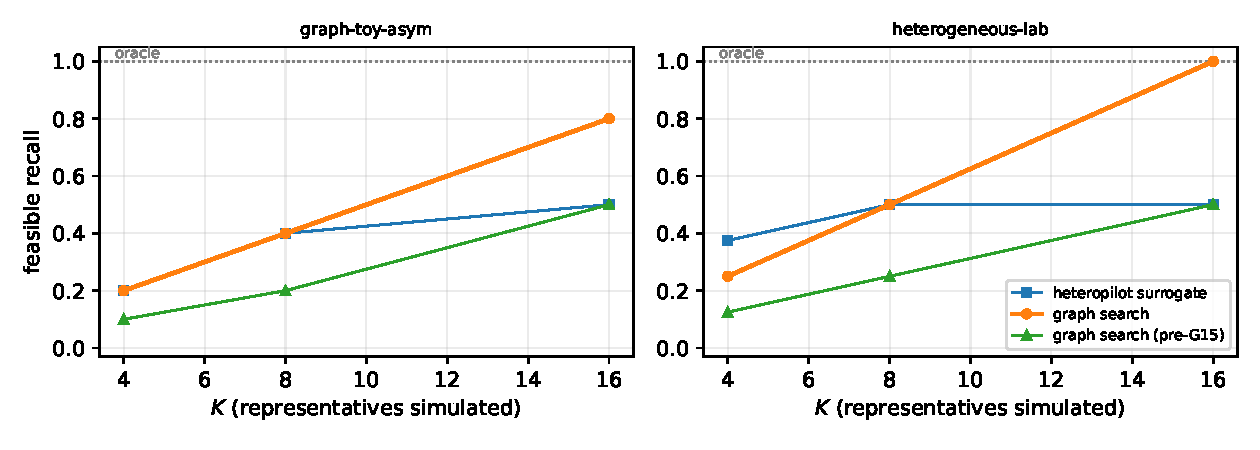
\includegraphics[width=\linewidth]{topk_holdout.pdf}
  \caption{Feasible recall against the simulation budget, both arms, on the holdout fixtures~\sourcetag{MOCK}. The oracle's level is the dotted line. At $K=4$ the graph search is behind, which the curve shows without the reader comparing two rows.}
  \label{fig:topk}
\end{figure}

Table~\ref{tab:e_g1b_topk} and Table~\ref{tab:e_g2_topk_holdout} report
feasible recall against the existing planner's surrogate top-$K$ under a
specification whose SLOs bind. At $K = 8$ and $K = 16$ this search reaches
higher recall. At $K = 4$ it does not---it ties on one holdout fixture and
trails on the other---and that is the row to read before the others.

The baseline is scored generously and deliberately so. It ranks and judges
templates rather than placements, so it cannot name which devices a candidate
occupies; one verdict is therefore credited to every placement of the template
it judged. There is no stricter reading that would be fair to it, and winning
on a technicality would not be winning.

% claim: C25
% claim: C26
\input{e_g7_holdout}
\input{e_g7_baseline_fairness}

Table~\ref{tab:e_g7_holdout} reports a holdout fixed before the scaling grid
ran: \egsevenHoldoutEmbeddings{} embeddings compressing to
\egsevenHoldoutReps{} representatives, both correctness numbers zero, and
higher recall than the surrogate at the registered operating point. The second
holdout---a hardware fixture with one uplink reservation altered---does not
exist, because the hardware campaign has not produced it. That row is reported
as not run rather than omitted, since an omitted row reads as a row that
passed. \pending{E-G5: real-lab holdout}

\subsection{The contention model against the wire}

% claim: C15
% claim: C16
\input{e_g4_microbench_2}
\begin{figure}[t]\centering
  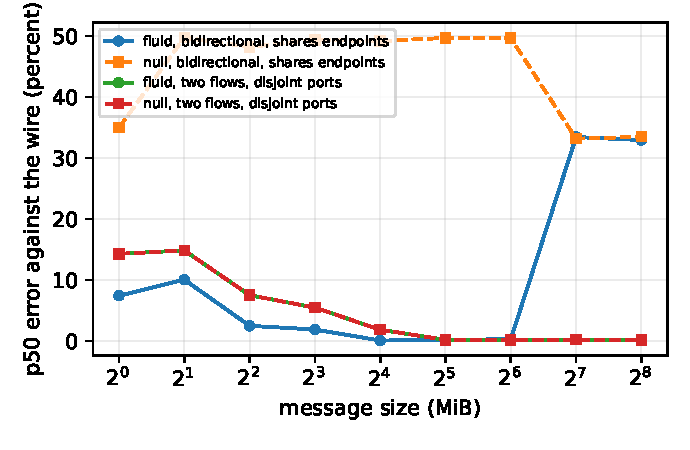
\includegraphics[width=\linewidth]{contention_error.pdf}
  \caption{Fluid and null error against message size, on the declaration the measurements support~\sourcetag{REAL HARDWARE}. The bidirectional error is near zero from 4 to 64 MiB and rises at 128: an accuracy domain, not a single figure.}
  \label{fig:contention}
\end{figure}

Table~\ref{tab:e_g4_microbench_2} reports the registered verdict, and it is a
\textbf{failure}: on the topology the plan declared before measuring,
processor-sharing is \egfourFluidPlannedSame\,\% out at the median on the
condition it exists for, against \egfourNullPlannedSame\,\% for pricing each
flow alone.

The reason is not the model. Two device pairs believed to share a host bridge
were measured to share nothing: each concurrent copy sustained the full
single-copy rate, and a third process saturating one pair left the other at its
unloaded rate to three digits. Run on the declaration the measurements support,
the same model is \egfourFluidMeasuredSame\,\% out; and on the bidirectional
condition, where the two flows genuinely do share endpoints, it is
\egfourFluidMeasuredBidi\,\% against \egfourNullMeasuredBidi\,\% for the null
model.

Both are reported because they are different corrections. One would rewrite the
contention model; the other rewrites a line of a cluster description. The
registered verdict is computed on the registered declaration, and the corrected
figure is not offered in its place.

% claim: C22
% claim: C29
\paragraph{The same question at a second location, with the opposite answer.}
Across an inter-node NIC between two machines, two concurrent streams take
exactly half each: a single stream reaches \egfourNicSingle~Gbit/s and two
reach \egfourNicTwoSame~each. That is processor sharing precisely, and it is
what the intra-node PCIe pairs did not do.

The pair of results is worth more than either alone. It is not that the model
is right in one place and wrong in another---it is that \emph{which resource
is genuinely shared} is a claim about hardware, settled by measurement at each
location separately, and the model prices whatever it is told to. The
bidirectional case says the same thing twice: the intra-node pair reaches only
a third again as much as a single direction, while the NIC exceeds twice it,
because that wire really is full duplex.

Two of the five registered conditions remain unanswered at this location, for
reasons that do not merge. Two concurrent flows over \emph{disjoint} NICs is
impossible on this hardware---each machine has exactly one InfiniBand
device---while the collective is deferred, needing an NCCL environment the peer
node does not yet have. \pending{E-G4: collective at location (b)}

% claim: C17
The model's accuracy domain has an upper end. Above a message size the hardware
begins overlapping the two directions of one link, the pair exceeds what
processor sharing predicts, and the model becomes optimistic by about a third.
That boundary is stated rather than absorbed into a fitted capacity: a capacity
chosen because it reproduces the answer is not a measurement, and it would make
the next node's prediction wrong silently.

\subsection{Hardware}

% pending
This section reports the deployment campaign: the recommended placement against
its SLOs, the boundary alternatives against the bounds that ranked or rejected
them, and the difference between two placements of one template across a shared
interconnect. The campaign is registered in the accompanying repository and has
not completed. \pending{E-G5: the hardware matrix}

% claim: C21
% pending
One result from it is already measured and is reported here because it does not
depend on the rest. Two placements of a single template---a tensor-parallel
pair on an NVLink link, and the same pair across a PCIe bridge---differ in
served $p99$ time to first token by a factor that grows sharply at the knee,
because the slower interconnect moves the knee itself. Three repetitions per
cell; the ranges do not overlap. The planner being extended cannot express the
difference between these two placements at all, which is the point.

%% Research design section 13 -- the five neighbouring systems, plus whatever
%% P6.4's fresh search turns up.
%%
%% Helix [R1], Vidur [R2], DistServe [R3], LLMServingSim 2.0 [R4],
%% Frontier [R5]. Two lines each, and both are required: what overlaps, and
%% what differs. A related-work entry with only the second is an advertisement.
%%
%% Section 13's prohibition applies with full force here: Helix already does
%% graph-based placement and scheduling, and heteropilot already has a Top-K.
%% The novelty claimed is the exact definition of redundancy, a compression that
%% does not lose the shared bottleneck, and quality management under a bounded
%% evaluation budget.
\section{Related work}
\label{sec:related}

\paragraph{Placement on heterogeneous clusters.}
Helix~\cite{helix} formulates serving over heterogeneous GPUs and network as a max-flow
problem and jointly optimises model placement and request scheduling. The
overlap is the object: it also represents the cluster as a graph, and this work
does not claim otherwise; nor does it contribute a scheduler. The difference is what the representation is used
for. Helix solves a flow problem to place and route; the search here
enumerates complete placements and folds them by exact equivalence so that an
expensive evaluator is invoked once per class, with the shared boundary in the
equivalence signature so that two placements crossing different contended links
are not folded together. Others search directly for a good configuration on
heterogeneous, decentralised or spot
GPUs~\cite{thunderserve,shuntserve,hexgen,melange,spotserve} or for a
parallelisation plan~\cite{alpa,galvatron}; this work contributes the
elimination discipline and the accounting of what was never evaluated.

\paragraph{Prefill--decode disaggregation.}
DistServe~\cite{distserve} separates the two phases onto different resources
and schedules them independently; Splitwise~\cite{splitwise},
TetriInfer~\cite{tetriinfer} and Mooncake~\cite{mooncake} disaggregate as well,
and Llumnix~\cite{llumnix} reschedules requests across engine instances. This
work generates disaggregated candidates and
prices the transfer between the phases as a flow over the graph, which is what
makes the counterexample in Section~\ref{sec:candidates} expressible at
all---two prefill groups sending to one decode group differ only in the uplink
they cross. It does not contribute a disaggregation policy, and the hardware
campaign deploys one only through its own experiment harness, because the
deployment backend of HeteroPilot~\cite{heteropilot} has no router
(Section~\ref{sec:limits}).

\paragraph{Simulation.}
Vidur~\cite{vidur} and LLMServingSim~\cite{llmservingsim,llmservingsim2}
provide simulators for LLM serving; Frontier~\cite{frontier,frontier2} argues
for more comprehensive and accurate simulation, including of disaggregated
architectures. The dependence here is direct---the evaluator is LLMServingSim
with an analytical backend---and so is the limitation: that simulator has no
representation of a link graph, so the evaluator sees a placement's own
bottleneck as a bandwidth but not which resources it shares.
Section~\ref{sec:adapter} reports what could not be expressed rather than
folding it into a bandwidth number.
This work measures search accuracy with prediction accuracy held fixed, which
is a different question from the one a simulator paper asks.

%% Research design section 12, "principal failure conditions", and section 11's invariants read
%% as a scope statement.
%%
%% Registered in docs/preregistration.md before the experiments ran, which is
%% what lets this section be written in the indicative rather than the
%% apologetic:
%%   - asymmetric clusters compress to ratio 1.0 by construction
%%     (graph-toy-asym is in the corpus so the number gets reported);
%%   - the isomorphism check can cost more than the simulation it saves, and
%%     the registered response is to demote exact compression to a cache key;
%%   - path-model error can dominate the ranking differences.
%%
%% Also here, and not buried: every fixture in this repository is fictional;
%% the contention model is fluid, not packet-level, and does not model
%% contention BETWEEN candidates; and a simulation at 128 devices is not a
%% hardware accuracy result.
\section{Limitations}
\label{sec:limits}

% claim: C4
\paragraph{The compression has a precondition.}
Exact equivalence folds placements only where the cluster has repeated
structure; on the toy asymmetric fixture it folds nothing (ratio
\egoneRatioAsym). Where the isomorphism check costs more than the simulation it
saves, the registered response is to demote exact compression to a cache key.

% claim: C13
% claim: C14
% claim: C40
\paragraph{Some placements never simulate.}
On the smallest corpus \egthreeUnjudgedLab{} of \egthreeEmbeddingsLab{}
placements returned no verdict, so the correctness result there is a
statement about the placements the simulator judged; on the toy corpora, once
the missing profile was measured, every placement was judged. Neither of the two causes
identified in Section~\ref{sec:eval} becomes a
verdict by being understood: the KV exhaustion is detected and raised, so the
failure carries a reason but not a verdict. With an A5000 decoding, the
simulator judged loads at which the hardware already preempts
(Section~\ref{sec:eval-pd}).

% claim: C34
% claim: C3
\paragraph{The simulator is told a placement's bandwidth, not what it shares.}
Every registered hardware prediction used the earlier adapter's first-pair
figure; the correction is evaluated only post hoc (Section~\ref{sec:eval-hw}).
Contention between a candidate's own flows on one port or NIC remains
invisible to the evaluator, and closing that needs a simulator with a link
graph. The same first-pair read remains in the compression's demand labels,
in the fluid model's choice of a flow's path and in the ranker's cut margin;
correcting them would change which candidates the registered runs reached, so
they are recorded rather than changed. For a tensor-parallel group of more
than two ranks, the labels and the earlier evaluator therefore shared one
blind spot, and the zero mis-merge count there is not independent evidence
that the labels are sufficient.

% claim: C22
% claim: C30
% claim: C39
\paragraph{Inter-node contention on a disaggregated deployment is smaller than
the model predicts.}
Inter-node \emph{P/D} runs---prefill on one node, decode on the other, the KV
pulled across the NIC by NIXL~\cite{nixl}---deployed by the experiment's own harness, because the
deployment backend of HeteroPilot~\cite{heteropilot} has no router. At a load the
configuration sustains, a background stream on the same NIC lengthened the
interval from prefill response to first decoded token by \egfivePdEffect{}
ms, with a standard deviation of \egfivePdSd{} ms over three pairs, so not
distinguishable from zero, where the fluid model predicted
\egfivePdPredicted{} ms: a ratio of \egfivePdRatio{}, outside the registered
agreement band. Across two accelerator types the two further directions miss
it too (Section~\ref{sec:eval-pd}). The model enters the background as a
standing reservation of its duty cycle; post hoc, a competing flow under
processor sharing brings one direction of three inside the band and leaves the
other two well below it. So the reservation is one wrong assumption, not the
only one, and nothing here separates the rest.

% claim: C38
% claim: C21
% not-established
\paragraph{Deferred by scope.}
On hardware only P/D crosses accelerator types, an A40 and an RTX A5000
(Section~\ref{sec:eval-pd}); every tensor-parallel group stays within one.
That the slower wire moves the load knee itself was seen only in the excluded
pilot runs and is not claimed. A burst-pattern defect was fixed before any
reported run. NPU deployment (no backend exists), a tensor-parallel group spanning two
accelerator vendors, KV-cache format conversion between them, learned rankers
and mixed parallelism degrees within one group are outside this work; nothing
here shows they cannot be done.

%% Research design section 13, the scope recommended for a first paper -- what this paper claims
%% and what it explicitly defers.
%%
%% In scope: intra-node homogeneous TP, inter-node heterogeneous replication,
%% and P/D where the runtime is confirmed to support it. Deferred and said so:
%% a single TP group spanning GPU and NPU, and KV-cache format conversion.
\section{Conclusion}
\label{sec:conclusion}

% claim: C24
% claim: C2
% claim: C11
% claim: C18
% claim: C30
% claim: C39
Placement is a decision a serving planner has to make and, enumerating over
islands, has no language for. This work gives it one: a relation that folds
only what a graph isomorphism confirms interchangeable, with the shared
boundary in the signature. Wherever an exhaustive oracle ran, no judged
feasible placement was wrongly removed and nothing differently priced was
folded, and under the real simulator the compression saved more time than it
cost. On
hardware, one plan at two of its placements is \egfiveTtwoOverTone{}x apart in
$p99$ time to first token at the load knee; on three inter-node directions
across two accelerator types, the contention model predicted far more slowdown
than the hardware showed, which is reported as a miss.


%% Where the references begin, for `make check-pdf`: the page this label lands
%% on is the first that does not count toward the venue's limit. Written at
%% shipout, so it is the page the label is actually set on. With no
%% bibliography after it the write rides on an empty page that is never
%% shipped, so the label is absent -- and check_pdf.py then counts every page,
%% which errs only toward failing.
%% Every float is set first: the venue's limit includes figures and tables, so
%% one deferred past this point would be content the count did not see.
\FloatBarrier
\makeatletter
\protected@write\@auxout{}{\string\newlabel{sec:refs}{{}{\thepage}}}
\makeatother
\bibliographystyle{IEEEtran}
\bibliography{refs}

\end{document}
